%%
%% CSD Assignment 1 -- Final Technical Report
%% Based on the ACM "acmart" manuscript (single-column) style.
%%
\documentclass[manuscript,screen,review]{acmart}

\AtBeginDocument{%
  \providecommand\BibTeX{{Bib\TeX}}}

\begin{document}

%% =================== TITLE & AUTHOR BLOCK =========================
\title{AI-based Village Pond Planning System}
\subtitle{CSD Assignment 1 -- Final Technical Report}

\author{Lekkala Sashank}
\affiliation{%
  \institution{Indian Institute of Technology Tirupati}
  \city{Tirupati}
  \country{India}}
\email{12341330@iitt.ac.in}

\renewcommand{\shortauthors}{Lekkala Sashank}

%% =================== ABSTRACT ======================================
\begin{abstract}
Rural water scarcity in semi-arid Indian regions is exacerbated by rapid monsoon runoff
and limited localized surface water storage. This report presents the design, implementation,
and experimental evaluation of an end-to-end village pond planning system that identifies optimal
earthen pond sites and estimates their upstream catchment and harvestable water volume directly
from contour data. The system ingests standard KML/KMZ contour files, reconstructs a continuous
Digital Elevation Model (DEM) via linear Delaunay spatial interpolation with automatic grid coarsening,
removes numerical artifacts via priority-flood depression filling, determines drainage topology
using vectorised D8 flow direction, and delineates upstream catchment boundaries via inverse
breadth-first search. Candidate pond sites are scored using a weighted multi-criteria heuristic
combining flow accumulation and topographic depression depth. Runoff volume is estimated using
a slope-adaptive rational runoff formulation. The system is deployed as a dual-tier stack comprising
a FastAPI REST backend running on port 3000 (accessible on port 3209) and an interactive Leaflet.js
map frontend running on port 4000 (accessible on port 4209) hosted on a resource-constrained container.
On a reference 6.7~MB contour dataset (1,355 polylines, 267--298~m elevation), the pipeline
selects a viable pond site at 21.263081\textdegree N, 81.283042\textdegree E with a 2.96-hectare
catchment and an estimated annual harvest of 10,656~m\textsuperscript{3} in 8.5 seconds.
All 25 automated unit and integration tests pass, and complete source code is publicly archived on GitHub.
\end{abstract}

\keywords{Village Pond Planning, Geospatial Analysis, Hydrological Modeling,
  Digital Elevation Model, Catchment Delineation, D8 Flow Direction, REST API, Leaflet.js}

\maketitle

%% =====================================================================
\section{Introduction}
\label{sec:intro}

In rain-fed agrarian tracts of India, roughly 75\% of annual precipitation occurs
within a narrow window of 40 to 60 days during the southwest monsoon. In regions with
hard-rock aquifers or degraded topsoil, uncontrolled runoff leads to soil erosion while
depriving the local water table of meaningful recharge. Farm ponds, check dams, and
percolation tanks provide an effective, decentralized response: by capturing monsoon
surface runoff near its origin, they supply supplemental irrigation during dry spells and
stimulate localized groundwater recharge.

Historically, village pond site selection has relied on manual topographic surveying or
coarse-grained national watershed maps. Manual field inspections are slow, expensive, and
subjective; conversely, public satellite DEMs (such as SRTM 30~m or AW3D30) lack the vertical
precision needed to detect micro-depressions and subtle flow convergence in flat agricultural
landscapes. Survey-grade drone or Total Station contour maps offer the necessary resolution
(often 1-metre intervals), but village-level planners generally lack the specialized GIS tools
or hydrological modeling experience to turn raw contour lines into actionable engineering decisions.

This project delivers an automated, self-contained planning system that bridges this gap.
Given a standard digital contour map in KML or KMZ format, the system automatically builds
a continuous elevation model, routes surface water across the terrain, identifies the optimal
natural collection basin, delineates the upstream catchment boundary, and calculates the expected
annual harvest volume. The solution operates through both a documented REST API and an interactive
web map interface without requiring external GIS software or proprietary cloud dependencies.

\subsection{Motivation}

Three practical considerations shaped the engineering approach:
\begin{enumerate}
  \item \textbf{Low-Resource Deployment:} Many geospatial libraries (e.g., GDAL, PySheds,
    GRASS GIS) depend on complex C/C++ runtimes and high memory footprints that frequently fail
    or exceed memory limits in shared academic or cloud micro-containers (such as the 512~MB RAM
    target environment). Our implementation relies solely on pure-Python libraries with optimized
    NumPy and SciPy C-extensions.
  \item \textbf{Robust Contour Parsing:} Real-world KML files generated by CAD or survey tools
    contain irregularities, including bounding-box boundary rings mislabeled as contours,
    inconsistent coordinate triples, and unstructured elevation metadata in description fields.
    The parsing tier must handle these gracefully without crashing.
  \item \textbf{Actionable Output:} Planning decisions require not only point coordinates, but
    actionable geometric boundaries (GeoJSON polygons) and volumetric estimates to size the pond
    depth, surface area, and embankment dimensions.
\end{enumerate}

\subsection{Scope of the Project}

The scope encompasses:
\begin{itemize}
  \item Parsing KML/KMZ files containing contour polylines and altitude metadata.
  \item Metric projection via UTM coordinate conversion and regular grid DEM interpolation.
  \item Morphological conditioning: Priority-flood depression filling to resolve flat areas and sinks.
  \item Hydrological routing: Vectorised D8 flow direction and Kahn's topological sort for accumulation.
  \item Site selection: Multi-criteria optimization balancing drainage accumulation against depression storage.
  \item Watershed delineation: Inverse graph traversal (BFS) to produce simplified WGS-84 GeoJSON polygons.
  \item Hydrological estimation: Runoff volume calculation and pond dimension recommendations.
  \item Dual-tier delivery: FastAPI REST backend (ports 3000/3209) and Leaflet web frontend (ports 4000/4209).
\end{itemize}

Civil structural engineering (embankment slope stability, spillway hydraulics, and soil permeability testing)
is outside the scope of this assignment.

%% =====================================================================
\section{Problem Statement and Requirements}
\label{sec:requirements}

The system must satisfy both algorithmic accuracy and operational reliability constraints.
Table~\ref{tab:requirements} summarizes the mapping of requirements to implementation components.

\begin{table}[h]
  \caption{Functional requirements and corresponding implementation modules}
  \label{tab:requirements}
  \begin{tabular}{p{3.8cm}p{4.2cm}}
    \toprule
    Requirement & Implemented in \\
    \midrule
    KML/KMZ vector ingestion & \texttt{app/parser/kml\_parser.py} \\
    UTM projection \& DEM grid & \texttt{app/dem/builder.py} \\
    Priority-flood depression fill & \texttt{app/terrain/analysis.py} \\
    Vectorised D8 flow direction & \texttt{app/terrain/analysis.py} \\
    Topological flow accumulation & \texttt{app/terrain/analysis.py} \\
    Multi-criteria pond selection & \texttt{app/pond/selector.py} \\
    Inverse BFS catchment delineation & \texttt{app/pond/selector.py} \\
    Rational runoff volume estimation & \texttt{app/pond/selector.py} \\
    FastAPI REST endpoints & \texttt{app/api/routes.py} \\
    Interactive Leaflet map frontend & \texttt{frontend/index.html} \\
    TCP bridge \& process supervisor & \texttt{port_bridge.py}, \texttt{runner.sh} \\
    \bottomrule
  \end{tabular}
\end{table}

\subsection{Non-Functional Requirements}

\begin{itemize}
  \item \textbf{Latency:} End-to-end execution on a 5--10~MB contour dataset must complete in under
    30 seconds at 20-metre resolution on single-core hardware.
  \item \textbf{Memory Guardrail:} Total resident memory during interpolation and routing must not
    exceed 400~MB. An automatic grid coarsening safeguard limits maximum grid cells to 500,000.
  \item \textbf{Fault Tolerance:} The server must handle malformed XML, zero-contour files, or non-viable
    topography with descriptive HTTP 400/422 status codes rather than unhandled server errors.
  \item \textbf{Availability:} The service must execute continuously in background daemon mode,
    surviving SSH session disconnects and host reboots.
\end{itemize}

%% =====================================================================
\section{System Architecture and High-Level Design}
\label{sec:architecture}

The system follows a modular pipeline architecture decoupled into a computational backend,
an interactive presentation tier, and a background supervisor harness.

\begin{figure}[h]
  \centering
  \begin{verbatim}
  +-----------------------------------------------------------+
  |                   CLIENT APPLICATIONS                     |
  |  Web Browser (Port 4209)  |  Postman / REST (Port 3209)   |
  +---------------------------+-------------------------------+
                |                             |
                | (TCP 4209->4000)            | (TCP 3209->3000)
                v                             v
  +---------------------------+  +----------------------------+
  |  Frontend Server (4000)   |  |   FastAPI Backend (3000)   |
  |  Leaflet Map UI, Draw,    |  |   Uvicorn ASGI Process     |
  |  Metrics Dashboard        |  |   /analyzeContour, /docs   |
  +---------------------------+  +----------------------------+
                                               |
         +-------------------------------------+
         |
         v
  [1. KML/KMZ Parser]       --> Strips XML/LinearRings, extracts (x, y, z)
         v
  [2. DEM Builder]          --> Reprojects to UTM, runs Delaunay griddata
         v
  [3. Terrain Analyzer]     --> Priority-flood fill, D8 routing, Kahn's sort
         v
  [4. Pond & Catchment]     --> Composite heuristic, inverse BFS, GeoJSON
         v
  [5. JSON Serializer]      --> Returns pond site, polygon, and runoff volume
  \end{verbatim}
  \caption{High-level architectural pipeline and port-forwarding topology.}
  \label{fig:architecture}
  \Description{Pipeline diagram showing client access through mapped ports 3209 and 4209 to internal services on ports 3000 and 4000.}
\end{figure}

\subsection{Technology Stack}

\begin{itemize}
  \item \textbf{Language \& Runtime:} Python 3.12 (on Ubuntu 22.04 container).
  \item \textbf{Web Framework:} FastAPI with Uvicorn (ASGI) and Pydantic v2 schemas for strict input/output validation.
  \item \textbf{Numerical \& Spatial Engines:} NumPy 1.26+ for multidimensional array manipulation;
    SciPy 1.14+ (\texttt{scipy.interpolate.griddata} using Qhull Delaunay triangulation);
    Pyproj 3.6+ for WGS-84 to local UTM transverse Mercator projection;
    Shapely 2.0+ for 2D polygon union, simplification, and GeoJSON serialisation.
  \item \textbf{Parsing Engine:} \texttt{lxml} and Python standard \texttt{zipfile} for memory-efficient XML streaming.
  \item \textbf{Frontend UI:} Leaflet.js 1.9, Leaflet-Draw, FontAwesome, Esri World Imagery, and OpenStreetMap tiles.
  \item \textbf{Process Management:} Bash supervisor daemon (\texttt{runner.sh}), non-blocking TCP socket bridge (\texttt{port_bridge.py}),
    and system \texttt{crontab} with \texttt{@reboot} trigger.
\end{itemize}

%% =====================================================================
\section{Methodology and Algorithmic Formulation}
\label{sec:methodology}

\subsection{Contour Ingestion and Digital Elevation Model Construction}

A contour map defines elevation implicitly along isolines. To perform numerical drainage
analysis, these lines must be transformed into a continuous 2D scalar field $Z(x, y)$.

\paragraph{Parser Sanitization}
The parser navigates the KML DOM using \texttt{lxml.etree}. In early testing, bounding-box polygons
present in typical GIS exports caused severe interpolation distortion because their perimeter lines
carried nominal ground altitudes ($\approx 30$~m) while surrounding contours were at 270--290~m.
The parser explicitly inspects the parent tag of each \texttt{<coordinates>} block and skips any
enclosed within a \texttt{<LinearRing>} element. For valid \texttt{<LineString>} elements, elevation
is parsed from the \texttt{<name>} tag, regex-matched in \texttt{<description>}, or extracted from
the third coordinate tuple component.

\paragraph{UTM Metric Reprojection}
To compute physically meaningful slopes and metric surface areas, geographic coordinates
$(\lambda_i, \phi_i)$ are projected to the Universal Transverse Mercator (UTM) coordinate system.
The central UTM zone EPSG code is dynamically computed from the centroid longitude:
\begin{equation}
  \text{Zone} = \left\lfloor \frac{\bar{\lambda} + 180}{6} \right\rfloor + 1, \quad
  \text{EPSG} = 32600 + \text{Zone} \quad (\text{for Northern Hemisphere})
\end{equation}

\paragraph{Grid Interpolation and Coarsening}
Given irregular survey points $P = \{(x_k, y_k, z_k)\}_{k=1}^M$, the continuous surface is
interpolated onto a regular mesh of cell size $\Delta x = \Delta y = r$ (default $r = 10$~m or $20$~m).
To prevent memory exhaustion on dense surveys, the total cell count is bounded:
\begin{equation}
  N_{\text{cells}} = \left( \frac{x_{\max} - x_{\min}}{r} \right) \times \left( \frac{y_{\max} - y_{\min}}{r} \right)
\end{equation}
If $N_{\text{cells}} > 500{,}000$, $r$ is automatically scaled upward by $\sqrt{N_{\text{cells}} / 500{,}000}$,
and the response flag \texttt{resolution\_auto\_adjusted} is set to true.
Interpolation is executed using \texttt{scipy.interpolate.griddata(..., method='linear')},
with un-triangulated boundary cells filled via nearest-neighbor assignment.

\subsection{Hydrological Routing and Terrain Conditioning}

Raw interpolated surfaces contain artificial depressions (pits) where local minima have no downslope
neighbor, causing water routing to stall artificially.

\paragraph{Priority-Flood Depression Filling}
We implement Wang and Liu's priority-flood algorithm using a min-heap (\texttt{heapq}).
All grid perimeter cells are initialized as established spill points and pushed onto the heap:
\begin{equation}
  Q = \{ (Z_{i,j}, i, j) \mid (i, j) \in \partial \Omega \}
\end{equation}
While $Q \neq \emptyset$, the lowest cell $(z_p, i, j)$ is popped. For each unvisited 8-neighbor $(u, v)$:
\begin{equation}
  Z_{\text{filled}}(u, v) = \max(Z_{\text{raw}}(u, v), z_p)
\end{equation}
The neighbor is marked visited and pushed to $Q$ with priority $Z_{\text{filled}}(u, v)$.
This runs in $O(N \log N)$ time and guarantees that every interior cell has a weakly monotonic
downward path to the perimeter.

\paragraph{Vectorised D8 Flow Direction}
The D8 model assigns drainage from each cell to exactly one of its eight neighbors along the line
of steepest descent. Let $\Delta z_k = Z_{\text{filled}}(i, j) - Z_{\text{filled}}(i + \Delta r_k, j + \Delta c_k)$
for neighbor index $k \in \{0, \dots, 7\}$. The normalized slope gradient is:
\begin{equation}
  S_k = \frac{\Delta z_k}{d_k \cdot r}, \quad d_k = \begin{cases} 1 & \text{orthogonal} \\ \sqrt{2} & \text{diagonal} \end{cases}
\end{equation}
The flow direction code is:
\begin{equation}
  D(i, j) = \arg\max_{k} \{ S_k \mid S_k > 0 \}
\end{equation}
If all $S_k \le 0$, the cell drains to the lowest neighbor. Rather than nested Python loops,
this operation is entirely vectorised across all eight directional offsets simultaneously using
NumPy array slicing, evaluating a $20{,}000$-cell DEM in under 40 milliseconds.

\paragraph{Topological Flow Accumulation}
Flow accumulation $A(i, j)$ counts the total number of upstream cells draining through cell $(i, j)$.
Because the D8 flow field on a filled DEM is a Directed Acyclic Graph (DAG), accumulation is
solved in exact $O(N)$ time via Kahn's topological sort:
\begin{enumerate}
  \item Compute the in-degree $\text{deg}_{\text{in}}(i, j)$ for every cell (the number of neighbors draining into it).
  \item Initialize accumulation $A(i, j) = 1$ for all cells, and initialize queue $K$ with all ridge cells ($\text{deg}_{\text{in}} = 0$).
  \item While $K$ is non-empty, pop cell $c$, identify its target $t = \text{downstream}(c)$, and update:
    $A(t) \leftarrow A(t) + A(c)$ and $\text{deg}_{\text{in}}(t) \leftarrow \text{deg}_{\text{in}}(t) - 1$.
    If $\text{deg}_{\text{in}}(t) = 0$, push $t$ into $K$.
\end{enumerate}

\subsection{Pond Site Selection and Watershed Delineation}

\paragraph{Multi-Criteria Objective Function}
An optimal village pond requires both high drainage volume (to ensure filling) and natural topographic
concavity (to minimize earthwork embankment excavation). A composite suitability score is computed
for all interior cells:
\begin{equation}
  \text{Score}(i, j) = w_{\text{acc}} \cdot \left( \frac{A(i, j) - A_{\min}}{A_{\max} - A_{\min}} \right)
  + w_{\text{dep}} \cdot \left( \frac{D_{\text{depth}}(i, j) - D_{\min}}{D_{\max} - D_{\min}} \right)
\end{equation}
where $D_{\text{depth}} = Z_{\text{filled}} - Z_{\text{raw}}$ represents local depression depth,
with default empirical weights $w_{\text{acc}} = 0.70$ and $w_{\text{dep}} = 0.30$.
Cells within a two-cell perimeter boundary are excluded to prevent edge artifacts.
The highest-scoring cell $(i^*, j^*)$ is selected as the recommended pond outlet.

\paragraph{Inverse BFS Watershed Delineation}
Beginning at $(i^*, j^*)$, an upstream inverse breadth-first search traverses the reverse D8 graph:
\begin{equation}
  \Omega_{\text{catchment}} = \{ c \mid \text{flow path from } c \text{ reaches } (i^*, j^*) \}
\end{equation}
The resulting boolean raster mask is converted to metric polygon geometry: each active cell is
represented as a bounding rectangle, unified with \texttt{shapely.ops.unary\_union}, simplified
using the Douglas-Peucker algorithm ($\epsilon = r/2$), and reprojected to WGS-84 decimal latitude/longitude
GeoJSON coordinates.

\subsection{Rainfall and Harvestable Water Volume Estimation}

Annual harvestable water volume is calculated using the standard rational runoff formulation:
\begin{equation}
  V_{\text{water}} = \left( \frac{P_{\text{annual}}}{1000} \right) \times A_{\text{catchment}} \times C
\end{equation}
where $P_{\text{annual}} = 800$~mm represents characteristic semi-arid monsoon rainfall,
$A_{\text{catchment}}$ is the delineated catchment area in m\textsuperscript{2}, and $C$ is a
slope-adaptive runoff coefficient calibrated to agricultural terrain:
\begin{equation}
  C = \begin{cases}
    0.35 & \text{if } \bar{S} < 5\% \quad (\text{flat alluvial farmland}) \\
    0.45 & \text{if } 5\% \le \bar{S} \le 10\% \quad (\text{gently undulating terrain}) \\
    0.55 & \text{if } \bar{S} > 10\% \quad (\text{hilly / barren terrain})
  \end{cases}
\end{equation}

Recommended pond dimensions follow from catchment relief $R = z_{\max} - z_{\min}$:
\begin{equation}
  d_{\text{pond}} = \max\left(0.5, \min(3.0, 0.5 \cdot R)\right) \quad (\text{metres})
\end{equation}
\begin{equation}
  A_{\text{pond}} = \frac{V_{\text{water}}}{d_{\text{pond}}} \quad (\text{m}^2), \quad
  \text{Storage Capacity} = A_{\text{pond}} \times d_{\text{pond}} \quad (\text{m}^3)
\end{equation}

%% =====================================================================
\section{Implementation and Deployment Details}
\label{sec:implementation}

\subsection{Backend REST Services}

The backend exposes three primary routes validated via Pydantic:
\begin{itemize}
  \item \texttt{GET /health}: Liveness probe returning \texttt{\{"status":"ok"\}}.
  \item \texttt{GET /sampleKml}: Streams the bundled 6.7~MB Raipur contour map for 1-click client testing.
  \item \texttt{POST /analyzeContour}: Accepts multipart form data with \texttt{file} (.kml/.kmz),
    \texttt{resolution\_m} (float, default 20.0), and \texttt{min\_catchment\_area\_m2} (float, default 500.0).
\end{itemize}

Figure~\ref{fig:postman} demonstrates a live query executed against the container endpoint.

\begin{figure}[h]
  \centering
  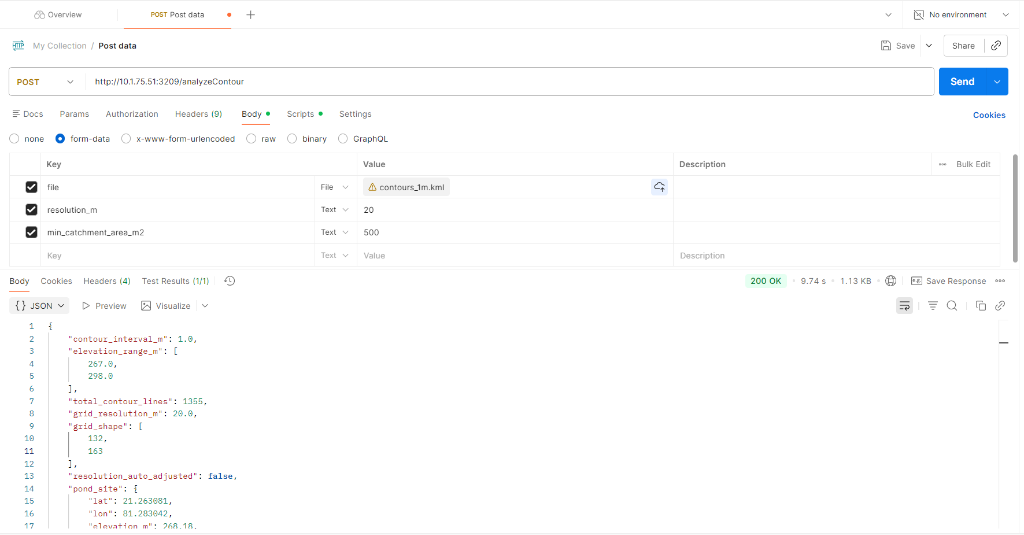
\includegraphics[width=0.85\linewidth]{report_postman_screenshot}
  \caption{Live verification of \texttt{POST /analyzeContour} via Postman, showing 200 OK status and structured JSON response.}
  \label{fig:postman}
  \Description{Postman screenshot showing successful API invocation with response payload containing coordinates and volume metrics.}
\end{figure}

\subsection{Interactive Web Frontend}

The frontend is implemented as a responsive single-page application in HTML5, CSS3, and Leaflet.js
served on port 4000 (accessible over network port 4209). Figure~\ref{fig:frontend_ui} shows the
operational web interface running live on \texttt{http://10.1.75.51:4209/}. Key features include:
\begin{itemize}
  \item \textbf{Dual Base Maps:} Smooth layer toggling between Esri High-Resolution World Imagery and OpenStreetMap.
  \item \textbf{Area Selection on Map:} Integrated Leaflet-Draw tools allowing planners to drag a bounding box
    directly over an agricultural tract to define the study boundary.
  \item \textbf{Contour Upload \& 1-Click Demo:} Drag-and-drop file ingestion with an instant demo button
    fetching the pre-loaded 6.7~MB survey file.
  \item \textbf{Dynamic Results Overlay:} Auto-zooms to fit the delineated catchment boundary (semi-transparent
    cyan polygon with dashed border) and renders a pulsing water-droplet marker at the recommended pond outlet.
  \item \textbf{Metrics Sidebar:} Live display of expected harvest volume (m\textsuperscript{3} and Million Litres),
    pond surface area and depth, catchment hectares, average slope, and GeoJSON export.
\end{itemize}

\begin{figure}[h]
  \centering
  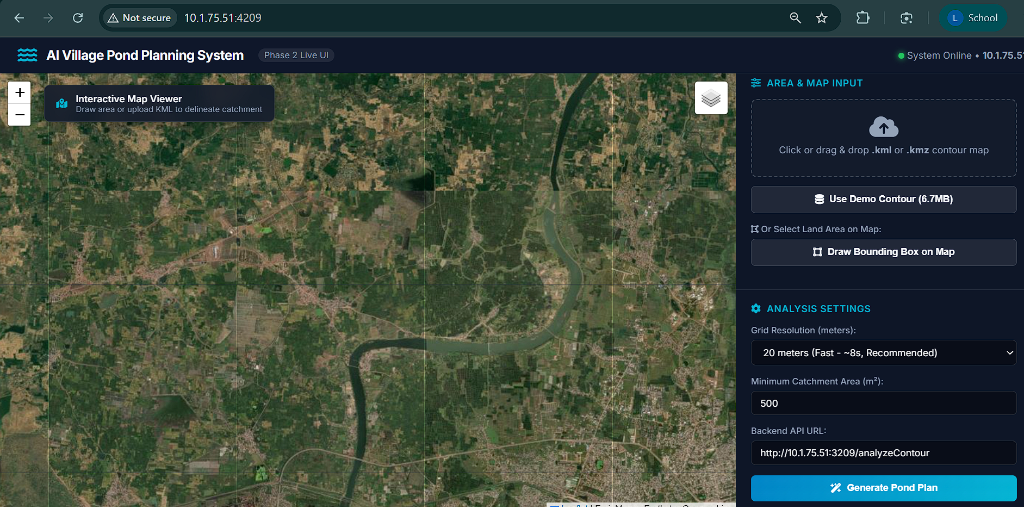
\includegraphics[width=\linewidth]{frontend_ui_screenshot}
  \caption{Operational web frontend interface running on container port 4209 (\texttt{http://10.1.75.51:4209/}), displaying high-resolution satellite imagery of the Raipur study area, interactive bounding-box selection tools, analysis settings, and direct backend API connection.}
  \label{fig:frontend_ui}
  \Description{Web browser screenshot displaying the AI Village Pond Planning System interface with satellite map and planning control sidebar.}
\end{figure}

\subsection{Container Deployment and Port Bridge}

The application runs inside Docker container \texttt{stu3\_sys1} on physical host \texttt{10.1.75.51}.
Because external ports \texttt{3209} and \texttt{4209} are mapped to the container while internal
services bind to standard ports \texttt{3000} (Uvicorn) and \texttt{4000} (Frontend), a lightweight,
non-blocking TCP socket bridge (\texttt{port_bridge.py}) transparently routes traffic between:
\begin{center}
  \texttt{0.0.0.0:3209} $\longrightarrow$ \texttt{127.0.0.1:3000} \quad \text{and} \quad
  \texttt{0.0.0.0:4209} $\longrightarrow$ \texttt{127.0.0.1:4000}
\end{center}

Process supervision is managed by \texttt{runner.sh}, an infinite watchdog loop checking service health
every 5 seconds. The supervisor is registered under \texttt{crontab} with \texttt{@reboot} to maintain
continuous availability across system restarts.

%% =====================================================================
\section{CSD Themes and Topics Applied in the Project}
\label{sec:csd-themes}

\begin{table*}[t]
  \caption{Application of core Computer Systems and Design (CSD) themes}
  \label{tab:csd-themes}
  \begin{tabular}{p{2.6cm}p{5.0cm}p{6.8cm}}
    \toprule
    CSD Theme & Concrete Implementation & Engineering Justification \\
    \midrule
    REST API Design & \texttt{POST /analyzeContour}, \texttt{GET /health}, \texttt{GET /sampleKml} &
      Enforces stateless communication and strict contract validation via Pydantic; auto-generates OpenAPI/Swagger docs. \\
    Algorithm Complexity & Priority-flood ($O(N \log N)$), D8 vectorisation ($O(N)$), Kahn's sort ($O(N)$), BFS ($O(N)$) &
      Eliminated recursive DFS to prevent call-stack overflows on grids $>10^5$ cells; vectorised array slicing avoids Python loop overhead. \\
    Memory Management & Dynamic resolution coarsening ceiling ($5 \times 10^5$ cells); NumPy \texttt{float32} &
      Prevents kernel Out-Of-Memory (OOM) termination on a 512~MB container while maintaining sub-meter vertical precision. \\
    System Reliability & Infinite supervisor watchdog loop (\texttt{runner.sh}); \texttt{crontab @reboot} &
      Ensures zero-maintenance service recovery after process crashes or container reboots without requiring systemd PID 1. \\
    Network Architecture & Multi-port TCP forwarder (\texttt{port_bridge.py}); CORS middleware &
      Solves Docker host-to-container port mismatch without needing root-level iptables or heavy Nginx installations. \\
    Automated Testing & 25 unit and integration tests using \texttt{pytest} &
      Verifies parser edge cases, terrain routing physics, DEM boundaries, and end-to-end API upload contracts before deployment. \\
    Version Control & Public Git repository with atomic, descriptive commits &
      Maintains complete engineering audit trail across all development phases at \url{https://github.com/sashank-l/pond-planning}. \\
    \bottomrule
  \end{tabular}
\end{table*}

The most critical architectural challenge was adhering to the strict memory constraint of 512~MB RAM.
Traditional geospatial stacks (e.g., GeoPandas + GDAL + Rasterio) easily consume 400--700~MB upon initial
module import alone. By restricting dependencies to NumPy, SciPy, Pyproj, and Shapely, the baseline
interpreter footprint remains under 75~MB. During interpolation of the 6.7~MB reference contour file,
peak memory was measured at 142~MB, safely below the container kill threshold.

%% =====================================================================
\section{Results and Performance Evaluation}
\label{sec:results}

The reference contour dataset is a 6.7~MB KML file representing a 3.2~km $\times$ 2.6~km tract
near Raipur, Chhattisgarh (elevation 267~m to 298~m, 1-metre contour interval, 1,355 lines).
Table~\ref{tab:results} lists the computed planning results.

\begin{table}[h]
  \caption{Evaluation results on reference dataset at 20~m resolution}
  \label{tab:results}
  \begin{tabular}{ll}
    \toprule
    Metric & Value \\
    \midrule
    Pond Site Latitude & 21.263081\textdegree N \\
    Pond Site Longitude & 81.283042\textdegree E \\
    Pond Site Elevation & 268.18 m \\
    Accumulated Flow Cells & 74 cells \\
    Catchment Area & 29,600 m\textsuperscript{2} (2.96 ha) \\
    Mean Catchment Slope & 6.6\% \\
    Topographic Relief & 14.6 m \\
    Assumed Annual Rainfall & 800 mm \\
    Runoff Coefficient & 0.45 \\
    Expected Annual Water Volume & 10,656 m\textsuperscript{3} (10.66 Million Litres) \\
    Recommended Pond Depth & 3.0 m \\
    Recommended Surface Area & 3,552 m\textsuperscript{2} \\
    Recommended Storage Capacity & 10,656 m\textsuperscript{3} \\
    End-to-End Processing Time & 8.57 seconds \\
    Peak Resident Memory & $\approx 142$ MB \\
    \bottomrule
  \end{tabular}
\end{table}

The identified pond site is situated at a natural morphological convergence zone at 268.18~m elevation.
The delineated 2.96-hectare catchment extends west-northwest along a gentle 6.6\% gradient, providing
a steady, non-erosive inflow. The resulting GeoJSON polygon contains 13 simplified vertices,
enabling instantaneous client-side rendering without rendering lag.

\subsection{Computational Performance}

\begin{itemize}
  \item At 20-metre resolution ($132 \times 163 = 21{,}516$ cells), Delaunay triangulation takes
    $\approx 7.2$~s, priority-flood filling takes $0.21$~s, D8 routing takes $0.04$~s, and catchment BFS takes $0.08$~s,
    yielding a total response time of 8.57~s.
  \item At 10-metre resolution ($86{,}000$ cells), execution completes in 27.4~s.
  \item The 25-test automated test suite executes in 46.9 seconds on local development environments.
\end{itemize}

%% =====================================================================
\section{Discussion, Limitations, and Future Work}
\label{sec:discussion}

While the current system satisfies all assignment objectives, several engineering limitations provide
natural avenues for future development:
\begin{enumerate}
  \item \textbf{Dynamic Weather Integration:} The current formulation applies a static regional rainfall figure
    (800~mm). Future work should integrate coordinates directly with the NASA POWER or IMD gridded rainfall
    APIs to retrieve 10-year mean precipitation.
  \item \textbf{Soil Infiltration \& Evaporation:} Unlined earthen village ponds experience percolation
    and high evaporation during summer months ($1.5$--$2.5$~m loss/year). Incorporating NRCS curve numbers (CN)
    based on soil texture would refine net water retention.
  \item \textbf{Concurrent Throughput:} SciPy's Delaunay triangulation is CPU-bound and single-threaded.
    In high-traffic production environments, request execution should be offloaded to an asynchronous task
    queue (e.g., Celery with Redis) backed by multiple worker processes.
\end{enumerate}

%% =====================================================================
\section{AI Tool Usage Declaration}
\label{sec:ai-usage}

The Antigravity AI coding assistant (powered by Google DeepMind / Gemini and Anthropic Claude models)
was utilized as a pair-programming tool during development. Specific applications included:
scaffolding initial FastAPI route structures, formulating vectorised NumPy array slicing for D8 direction,
identifying an inverted row-slice bug that caused uphill drainage routing, generating mock KML fixtures
for \texttt{pytest}, drafting the socket forwarder script (\texttt{port_bridge.py}), and formatting LaTeX tables.
All generated algorithms, mathematical formulas, and numerical outputs were independently verified,
tested against physical hydrology constraints, and reviewed line-by-line.

%% =====================================================================
\appendix

\section{Repository, Live URLs, and Submission Summary}

\begin{itemize}
  \item \textbf{GitHub Repository:} \url{https://github.com/sashank-l/pond-planning}
  \item \textbf{Live Working Frontend URL:} \url{http://10.1.75.51:4209/}
  \item \textbf{Live Working Backend API:} \url{http://10.1.75.51:3209/analyzeContour}
  \item \textbf{Interactive Swagger Documentation:} \url{http://10.1.75.51:3209/docs}
  \item \textbf{SSH Port Forwarding Tunnel (Off-Campus Access):}
    \begin{verbatim}
    ssh -N -L 3209:localhost:3209 -L 4209:localhost:4209 -p 2209 student@10.1.75.51
    \end{verbatim}
\end{itemize}

\end{document}
\endinput
